\section{Geometry Generation}

% TODO Adds birds-eye view of the house to show the plane of symmetry

Designing a good model geometry is critical as it can save significant computational resources.
When designing a geometry the FEM user should try to represent the model geometry as accurately as possible while:
\begin{enumerate}
  \item Avoid unnecessarily fine details; these may require an excessively fine mesh to resolve.
  \item Leverage symmetry to reduce geometry size and thereby the mesh.
\end{enumerate}\par
Achieving these goals is not always straightforward, and depend on the skill of the modeler and on the available tools.
Typically a model geometry is constructed in some computer assisted design (CAD) software, and the particular tools available in these vary by software.\par

COMSOL has a built-in geometry generation tool, which allows the construction of advanced geometries by performing various operations on simpler geometries, e.g. a cylinder and half sphere can be combined to make a rivet.
It is also possible to import pre-generated geometries from other CAD software.
However, we will create our own geometry.\par

The interior of the house itself will not be explicitly modeled, instead we only consider the soil surrounding the house.
This is done for the simple reason that it is not important to do so.
Once the contaminant is in the structure, that is the key consideration.
In addition, interiors are simply too heterogenous to generalize in any meaningful way.
If the interior was explicitly modeled to offer insights into indoor concentration variations, it would be prohibitively expensive to do, as it would require solving the Navier-Stokes equation.
Instead the interior is implicitly modeled as a CSTR and simply coupled with the explicit soil and foundation geometry via the foundation crack boundary.\par

One of the nice properties of our VI scenario is that, due to symmetry, we only need to explicitly model a quarter of it.
This reduces the number of required mesh points by 75\%, which is a huge computational saving.
To create the specified geometry, see the instructions for geometry generation in the appendix.

\begin{figure}[htb!]
  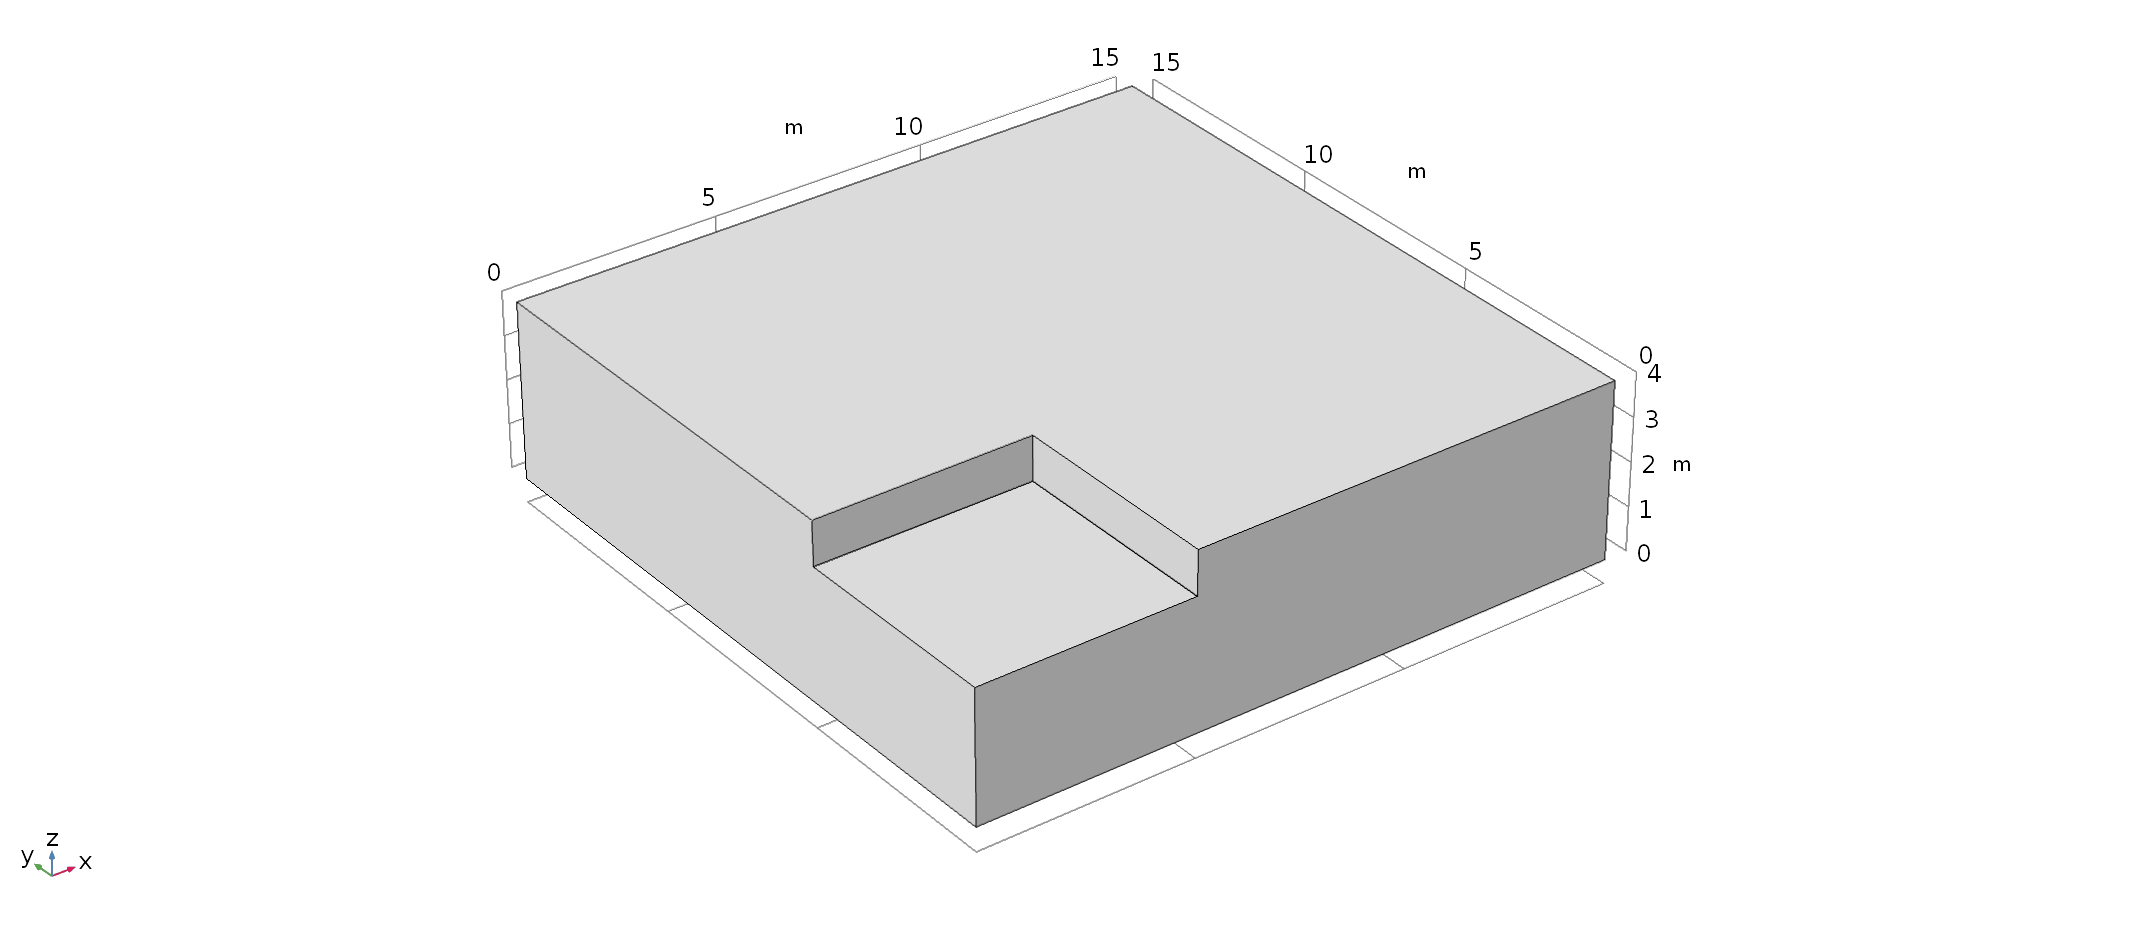
\includegraphics[width=\textwidth]{vi_model.png}
  \caption{The complete geometry of the VI scenario.}
  \label{fig:geometry}
\end{figure}
